\chapterimage{images/recycler/recycling.jpg}
\chapter{Recyclerview}
In 2014, Google released RecyclerView , via the Android Support package.
Developers can add the recyclerview-v7 to their projects and use RecyclerView. In this chapter, we will review RecyclerView from the ground up, starting with basic
operation.

\section{What is a recyclerview}
The RecyclerView is a new ViewGroup that is prepared to render any adapter-based view. It is supposed to be the successor of ListView and GridView, and it can be found in the latest support-v7 version. One of the reasons is that RecyclerView has a more extensible framework, especially since it provides the ability to implement both horizontal and vertical layouts. Use the RecyclerView widget when you have data collections whose elements change at runtime based on user action or network events.

To use a recyclerview, you will need the following things:
\begin{enumerate}
	\item RecyclerView.Adapter - To handle the data collection and bind it to the view
	\item LayoutManager - Helps in positioning the items
	\item ItemAnimator - Helps with animating the items for common operations such as Addition or Removal of item
\end{enumerate}
This is on top of the adapters and view holders that were the hallmarks of
conventional AdapterView usage.

\section{Components and Workflow}

\begin{figure}
	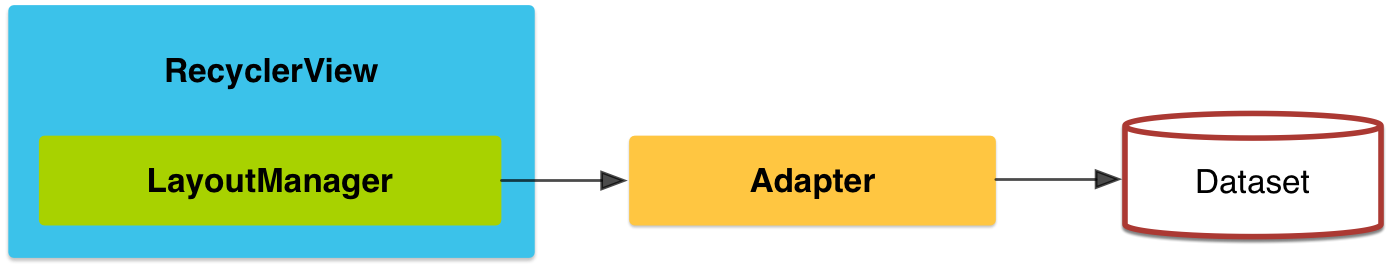
\includegraphics[width=\textwidth]{images/recycler/components.png}
	\caption{ RecyclerView is a major enhancement over ListView. It contains many new features like ViewHolder, ItemDecorator, LayoutManager, and SmoothScroller. But one thing that certainly gives it an edge over the ListView is; the ability to have animations while adding or removing an item. }
	\label{fig:recyclercomponents}
\end{figure}

\subsection{LayoutManagers}
After adding a recyclerview to the activity, the first thing we do is call setLayoutManager() ,
which will associate a RecyclerView.LayoutManager with our RecyclerView, for example a LinearLayoutManager. RecyclerView
knows absolutely nothing about how to lay out its children. That work is delegated
to a RecyclerView.LayoutManager , so that different approaches can be plugged in as
needed.

There are three concrete subclasses of the abstract RecyclerView.LayoutManager
base class that ship with recyclerview-v7 :
\begin{enumerate}
	\item LinearLayoutManager , which implements a vertically-scrolling list
	\item GridLayoutManager ,
	which implements a two-dimensional vertically-
	scrolling list
	\item StaggeredGridLayoutManager , which implements a “staggered grid”, which
	has columns of cells like a GridView , but where the cells do not have to all
	have the same size.
\end{enumerate}







\subsection{RecyclerView.Adapter}
RecyclerView uses an adapter to help convert our model data
into visual representations. A RecyclerView.Adapter  uses a generic to
identify a ViewHolder that will be responsible for doing the work to actually tie
model data to row widgets.

RecyclerView.Adapter has three abstract methods that need to be implemented.

\begin{enumerate}
	\item getItemCount() , which fills the same role as does getCount() indicating how many items there will be in the RecyclerView
	\item onCreateViewHolder()  needs to create, configure,
	a ViewHolder for a particular row of our list. It is passed two parameters:
	\begin{enumerate}
		\item a ViewGroup that will hold the views managed by the holder, mostly for use
		with layout inflation, and
		\item an int that is the particular view type we are using, for cases where we have
		multiple view types
	\end{enumerate}
	\item onBindViewHolder()
	is responsible for updating a ViewHolder based upon the
model data for a certain position .
\end{enumerate}


\subsection{ViewHolder}
The RecyclerView.ViewHolder is responsible for binding data as needed from our
model into the widgets for a row in our list. However, other than needing to use the base class of RecyclerView.ViewHolder ,
there is no other particular protocol that is mandated between the adapter and the
view holder. You can invent your own API.

\subsection{ItemAnimator}
RecyclerView.ItemAnimator will animate ViewGroup modifications such as add/delete/select that are notified to adapter. DefaultItemAnimator can be used for basic default animations and works quite well.


\subsection{Responding to Clicks}
At its core, responding to clicks is a matter of setting an OnClickListener on the
appropriate Views, in this case the ViewHolder. 




\section{CardView}
ards are a popular visual metaphor in mobile development. Dividing content
collections (or aspects of a larger piece of content) into cards makes it clearer how you can reorganize that content to fit various screen sizes and orientations. In some
cases, you might have a single column of cards, while in other cases, you have cards
arranged more laterally.

In 2014, Google released cardview-v7 , another library in the Android Support
package, that offers a CardView . CardView is a simple subclass of FrameLayout ,
designed to provide a card UI, consisting of a rounded rectangle and a drop shadow.
In particular, CardView will use Android 5.0’s default drop shadows based on widget
elevation, while offering emulated drop shadows on earlier Android releases. This
way, you can get a reasonably consistent look going back to API Level 7.
To use this, you will have to add the cardview-v7 library to your app project.
Android Studio users can just add a dependency on the cardview-v7 artifact in the
Android Support repository
